Arduino er en opensource plattform som inneholder både Arduino brett og Arduino kodespråk (basert på Wiring). 
Arduinoen brukt i dette prosjektet er en Arduino Nano (figur \ref{fig:arduino-nano}), som er basert på mikrokontrolleren ATmega328. 
Koden skrives i Arduino sin egen IDE, som også brukes til å laste opp kode og monitorere data fra Arduinoen. \parencite{ArduinoNano} 
I dette prosjektet blir Arduinoen brukt som en adapter mellom Pozyx tagen og Pixhawk flightcontrolleren. 
Den leser av avstandene til ankrene fra tagen, og sender denne informasjonen til pixhawken via MavLink.

\begin{figure}[htp]
    \centering
    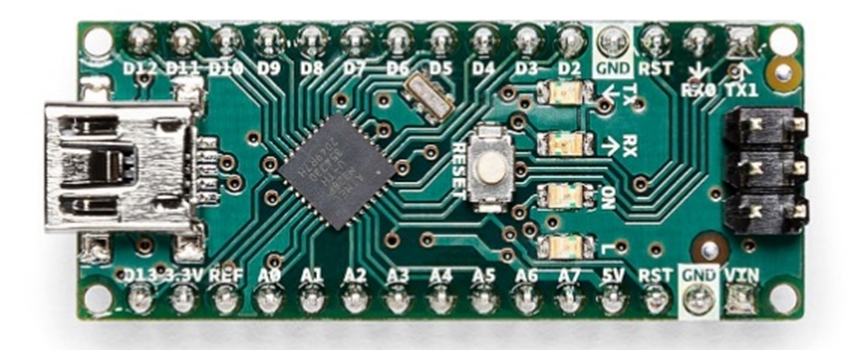
\includegraphics[width=0.5\columnwidth]{figures/arduino-nano}
    \caption{Arduino nano.\parencite{ArduinoIntroduction}}
    \label{fig:arduino-nano}
\end{figure}
    